\chapter{Hasil dan Pembahasan} \label{bab4}
\section{Hasil Pengujian}
Setelah melaksanakan pengujian sistem seperti yang telah dibahas pada bab sebelumnya sub bab ini akan memaparkan hasil dari percobaan.
\subsection{Jumlah Fitur Sistem}\label{hasil:jumlahfitur}
%\subsubsection{Pemantauan dan Deteksi}
Pemantauan (aktivitas jantung) dan Deteksi (detak dan aritmia) berhasil dilakukan secara realtime (parameter lainnya, dibahas pada sub bab berikutnya). Berikut perbandingan mode \textit{monitoring} pada sistem di Tugas Akhir ini dengan sistem sejenis lainnya yang berada pada puncak 10 Android Playstore (kata pencarian heart rate) \cite{playstore_heart}.

\begin{table}[H]
	\centering
	\begin{tabular}{|l|L{5cm}|c|L{0.5cm}|L{0.5cm}|L{0.5cm}|L{0.5cm}|L{0.5cm}|L{0.5cm}|L{0.5cm}|L{0.5cm}|}
		\hline
		\rowcolor{gray}
		\textbf{No} & \textbf{Produk} & \textbf{Sen} & \multicolumn{8}{c}{\textbf{Fitur}} \\
		\rowcolor{gray}
		 & & \textbf{sor} & A & B & C & D & E & F & G & H \\
		\hline
		1 & Instant Heart Rate : Heart Rate \& Pulse Monitor & PPG & Y & N & Y & Y & N & Y & N & Y \\
		2 & iCare Health Monitor (BP \& HR) & PPG & Y & N & Y & N & N & Y & N & Y \\
		3 & Heart Rate Monitor(REPS) & PPG & Y & N & Y & Y & N & Y & N & Y \\
		4 & Runtastic Heart Rate Monitor \& Pulse Checker & PPG & Y & N & Y & N & N & Y & N & N \\
		5 & Cardiograph - Heart Rate Meter & PPG & Y & N & Y & Y & N & Y & N & Y \\
		6 & ASUS Heart Rate & PPG & N & N & N & N & N & Y & N & N \\
		7 & Samsung Health & PPG & Y & Y & N & N & N & Y & N & Y \\
		8 & Heart Rate Monitor(Meet Your Need Production) & PPG & N & N & N & N & N & Y & N & N \\
		9 & MobECG & ECG & N & Y & Y & Y & N & Y & N & N \\		
		10 & CMS50Dplus & ECG & N & Y & Y & Y & N & Y & N & N \\
		\hline
		\textbf{*} & \textbf{Tugas Akhir} & \textbf{PPG} & \textbf{Y} & \textbf{Y} & \textbf{Y} & \textbf{Y} & \textbf{Y} & \textbf{Y} & \textbf{Y} & \textbf{Y} \\
		\hline
	\end{tabular}
\end{table}

Ket: \\
A = Identitas User \\
B = Real Time Monitoring \\
C = Melihat Gelombang Jantung \\
D = Merekam Gelombang Jantung \\
E = Multiuser Monitoring \\
F = Deteksi BPM \\
G = Aritmia Alert \\
H = Share Result via Network\\

\subsection{Delay}
Pengujian dilakukan oleh pengguna yang bergerak secara bebas dalam wilayah cakupan router (\textit{DAU}, \textit{router} dan \textit{SPU} masih dalam satu wilayah) sehingga tidak ada proses routing antara router. Setelah melakukan pengujian sebanyak 10 kali didapatkan rata-rata delay sekitar 1.72541 ms. Hasil rata rata pengukuran delay tiap 10 detik dalam 1 menit tertera pada gambar \ref{fig:delay}. Tabel pengukuran delay yang lengkap terlampir pada lampiran \ref{lampiran:delay}.

\begin{figure}[H]
	\centering
	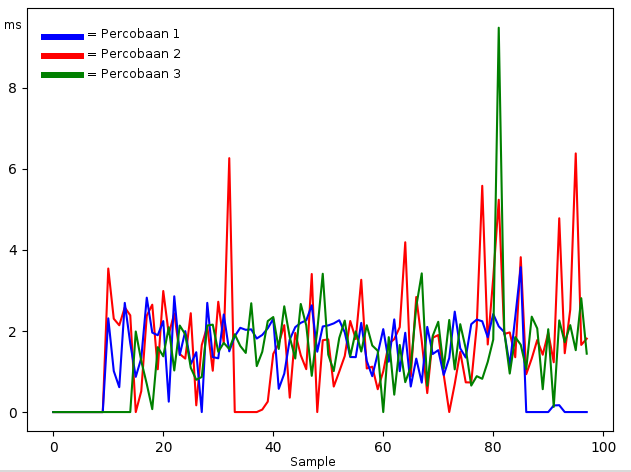
\includegraphics[scale=0.5]{images/delay1.png}
	\caption{Hasil Pengukuran Delay 100 sample}
	\label{fig:delay}
\end{figure}

\subsection{Execution Time}
\textit{Execution Time} perlu diukur pada 2 lokasi yaitu \textit{DAU} dan \textit{SPU}. Hal ini ditujukan untuk mengetahui \textit{maximum sampling speed} yang mungkin dilakukan pada \textit{DAU} sebelum terjadi \textit{bottleneck}. 

Pengujian pada \textit{DAU} dilakukan sebanyak 10 kali. Berdasarkan pengujian, didapatkan rata-rata waktu eksekusi ialah \exec ms per sampel. Hasil rata rata pengukuran waktu eksekusi tiap 10 detik dalam 1 menit tertera pada gambar \ref{fig:exec_time}. Tabel pengukuran waktu eksekusi pada DAU yang lengkap terlampir pada lampiran \ref{lampiran:exec_time}.

Pengujian pada \textit{SPU} dilakukan sebanyak 10 kali. Berdasarkan pengujian, didapatkan rata-rata waktu eksekusi ialah \execs ms per sampel. Hasil rata rata pengukuran waktu eksekusi tiap 10 detik dalam 1 menit tertera pada gambar \ref{fig:exec_time2}. Tabel pengukuran waktu eksekusi pada SPU yang lengkap terlampir pada lampiran \ref{lampiran:exec_time}.

\begin{figure}[H]
	\centering
	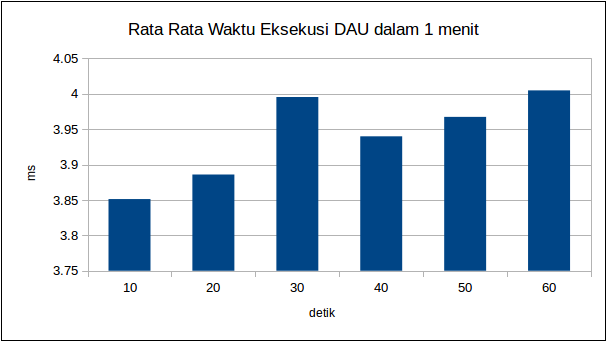
\includegraphics[scale=0.5]{images/exec_time1.png}
	\caption{Hasil Pengukuran Waktu Eksekusi Pada DAU}
	\label{fig:exec_time}
\end{figure}

\begin{figure}[H]
	\centering
	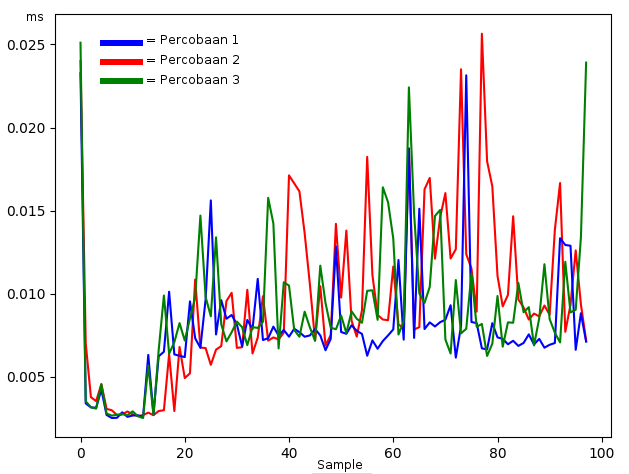
\includegraphics[scale=0.5]{images/exec_time2.png}
	\caption{Hasil Pengukuran Waktu Eksekusi Pada SPU}
	\label{fig:exec_time2}
\end{figure}

%\subsection{FPS}
%FPS umumnya ditentukan oleh kapasitas \textit{hardware} yang me-\textit{render} tampilan, namun untuk memaksimalkan jumlah \textit{CMU}, satu nilai FPS perlu dipilih untuk dijalankan pada semua \textit{CMU}. Berikut hasil lengkap percobaan FPS yang dilakukan pada \textit{CMU} web dan android.

%\begin{table}[H]
%	\centering
%	\begin{tabular}{|l|L{4cm}|L{4cm}|}
%	\rowcolor{gray}
%	\textbf{FPS} & \textbf{Web} & \textbf{Android} \\
%	\hline
%	10 & Grafik Patah Patah tapi lancar & Grafik Patah Patah tapi lancar \\
%	\hline
%	20 & Grafik Patah Patah tapi lancar & Grafik halus dan lancar \%\
%	\hline
%	30 & Grafik halus dan sekali kali \textit{freeze} & Grafik halus dan sekali kali \textit{freeze} \\
%	\hline
%	40 & Grafik halus tapi sekali kali \textit{freeze} & Grafik halus tapi sering \textit{freeze} \\
%	\hline
%	50 & Grafik halus tapi sering \textit{freeze} & Grafik halus tapi sering \textit{freeze} \\
%	\hline
%	\end{tabular}
%\end{table}

\subsection{Akurasi}
Setelah melakukan pengujian didapatkan hasil akurasi 99\% untuk detaksi detak dan \accuracy untuk deteksi aritmia.
\subsubsection{a. Akurasi Deteksi Puncak}
Dilakukan percobaan untuk menemukan konfigurasi konstanta deteksi $d$ (durasi window), $\alpha$ (\textit{peak threshold, val by mean}), dan $\beta$ (\textit{min distance threshold, idx by R}). Skenario percobaan variabel dapat dilihat pada tabel \ref{table:experiment_var}. Hasil percobaan tersebut dapat dilihat pada tabel \ref{table:exec_time3}. Sebagai perbandingan kolom skenario \textit{original} pada tabel \ref{table:exec_time3} merupakan hasil percobaan menggunakan algoritma Pan-Tompkins yang asli.

\begin{table}[H]
	\centering
	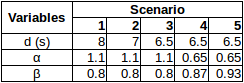
\includegraphics[scale=0.8]{images/experiment_variable.png}
	\caption{Variabel eksperiment}
	\label{table:experiment_var}
\end{table}

\begin{table}[H]
	\centering
	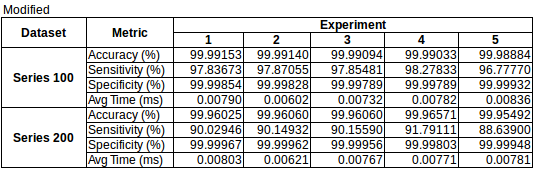
\includegraphics[scale=0.75]{images/modif_beat_detect.png}	
	\caption{Hasil Pengujian Algoritma Deteksi Detak Jantung pada Python}
	\label{table:exec_time3}
\end{table}

Perbandingan antara algoritma modifikasi dengan algoritma pantom yang asli dapat dilihat pada diagram batang \ref{fig:compare_performance_100}, \ref{fig:compare_performance_200} dan \ref{fig:compare_exec}.

\begin{figure}[H]
	\centering
	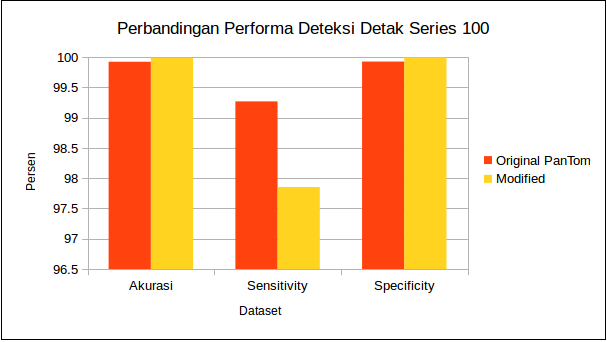
\includegraphics[scale=0.65]{images/beat_perform_100.png}
	\caption{Perbandingan Performa Deteksi Data Series 100}
	\label{fig:compare_performance_100}
\end{figure}
\begin{figure}[H]
	\centering
	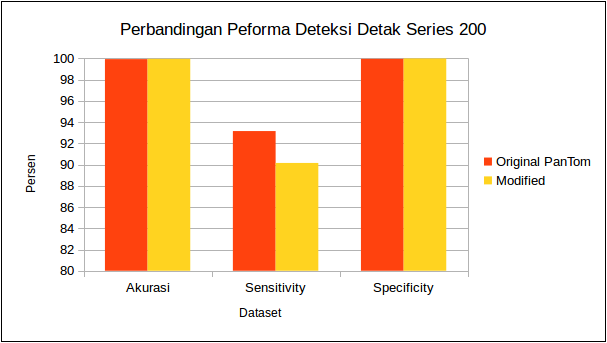
\includegraphics[scale=0.65]{images/beat_perform_200.png}
	\caption{Perbandingan Performa Deteksi Data Series 200}
	\label{fig:compare_performance_200}
\end{figure}
\begin{figure}[H]
	\centering
	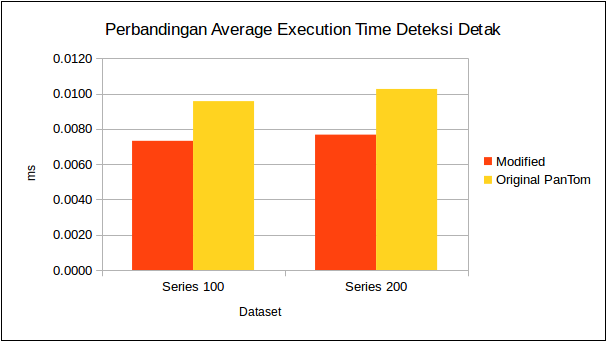
\includegraphics[scale=0.65]{images/beat_exec.png}
	\caption{Perbandingan Waktu Akurasi}
	\label{fig:compare_exec}
\end{figure}

\subsubsection{b. Akurasi Deteksi Aritmia}
Pengujian akurasi deteksi aritmia terbagi menjadi 3 bagian. Pengujian pertama, sistem deteksi menerima inputan detak jantung asli sesuai data dari MIT BIH. Pengujian kedua, sistem deteksi menerima inputan detak jantung hasil deteksi tahap sebelumnya dengan algoritma asli dari PanTomkins. Pengujian ketiga, sistem deteksi menerima inputan detak jantung hasil deteksi tahap sebelumnya dengan algoritma modifikasi dari PanTomkins.Hasil pengujian tertera pada tabel \ref{fig:aritmia_compare} merupakan hasil percobaan menggunakan algoritma Pan-Tompkins yang asli. Untuk mempermudah pemahaman hasil pengujian juga dapat dilihat dalam diagram batang pada gambar \ref{fig:aritmia_accuracy}, \ref{fig:aritmia_sensitivity}, dan \ref{fig:aritmia_specificity}.

\begin{table}[H]
	\centering
	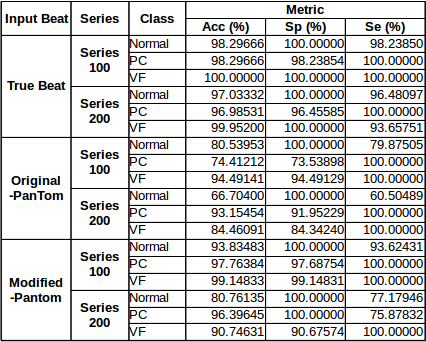
\includegraphics[scale=0.7]{images/aritmia_compare.png}
	\caption{Tabel Performa deteksi Aritmia dengan input berbeda}
	\label{fig:aritmia_compare}
\end{table}

\begin{figure}[H]
	\centering
	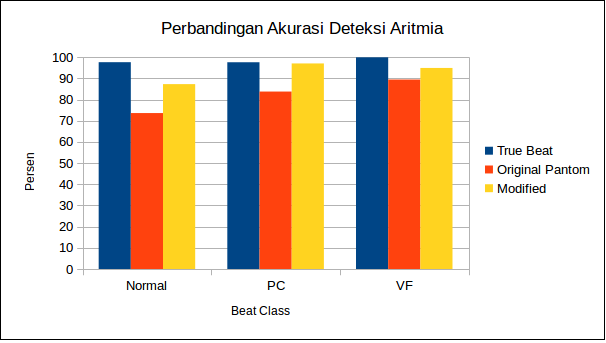
\includegraphics[scale=0.7]{images/aritmia_acc.png}
	\caption{Perbandingan akurasi deteksi Aritmia dengan input berbeda}
	\label{fig:aritmia_accuracy}
\end{figure}
\begin{figure}[H]
	\centering
	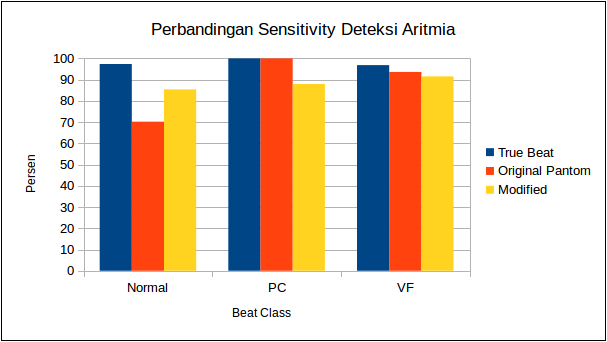
\includegraphics[scale=0.7]{images/aritmia_se.png}
	\caption{Perbandingan sensitvitas deteksi Aritmia dengan input berbeda}
	\label{fig:aritmia_sensitivity}
\end{figure}
\begin{figure}[H]
	\centering
	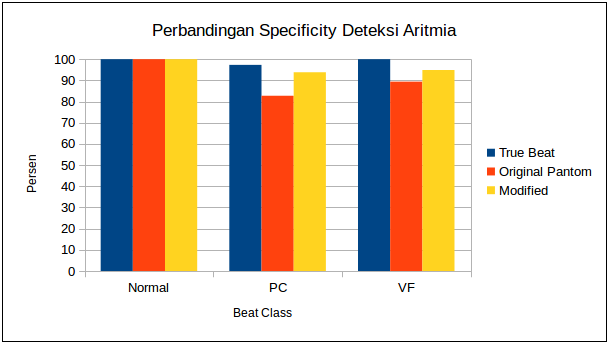
\includegraphics[scale=0.7]{images/aritmia_sp.png}
	\caption{Perbandingan spesifisitas deteksi Aritmia dengan input berbeda}
	\label{fig:aritmia_specificity}
\end{figure}

\section{Pembahasan}\label{bab4:pembahasan}
Dengan pengimplementasian rancangan arsitektur, sistem yang dibangun dapat memiliki semua fitur yang dimiliki sistem sejenis (\ref{hasil:jumlahfitur}). Delay yang terjadi selama pengiriman sampel selalu berubah ubah namun memiliki rata rata \delay. Perubahan nilai delay terjadi karena pengaruh kehandalan jaringan (WiFi) dan subjek yang bebas bergerak. 

Waktu eksekusi diukur pada \textit{DAU} dan \textit{SPU}. Pada \textit{DAU} terlihat waktu eksekusi yang berubah ubah (lihat gambar \ref{fig:exec_time}), ini dipengaruhi oleh adanya \textit{interupt} pengambilan sampel, pembuatan dan pengiriman paket, dan \textit{buffer memory management}. Sebagai perbandingan, tanpa melakukan pengiriman waktu eksekusi hanya selama 0.001 ms (waktu untuk mengambil sampel). Karena rata rata waktu eksekusi pada \textit{DAU} ialah \exec maka maksimum frekuensi sampel ialah 200Hz, atau setara dengan 1 sampel/5ms. 

Sedangkan pada \textit{SPU}, terlihat waktu eksekusi sangat tinggi pada permulaan kemudian sangat rendah lalu berfluktuasi (lihat gambar \ref{fig:exec_time2}), hal ini disebabkan oleh SPU yang membutuhkan waktu lebih lama untuk memulai \textit{subprocess} untuk tiap \textit{DAU} yang terhubung. Kemudian, tiap proses mengisi buffer hingga terisi untuk dilakukan operasi deteksi. Penggunaan Node.JS sebagai SPU juga memberikan dampak dalam kecepatan. Dibandingkan dengan Python, Node.JS dapat bekerja hampir 3 kali lebih cepat (gambar \ref{table:exec_time3}). Karena maksimum frekuensi sampel yang dapat diterapkan ialah 1 sampel tiap 5ms dan waktu eksekusi 1 sampel ialah \execs maka secara matematis SPU dapat memproses sekitar \sensor device secara bersamaan (maksimum total sensor dan CMU yang terhubung, 5ms / \execs).

Pada segi performansi, algortima deteksi puncak R terlihat hasil modifikasi menghasilkan akurasi, \textit{specificity} dan \textit{sensitivity} yang hampir menyamai algoritma pantomkins yang asli bahkan cenderung lebih baik (kecuali sensitivity) (lihat gambar \ref{fig:compare_performance_100} dan \ref{fig:compare_performance_200}). Hal ini secara langsung berdampak pada performa algoritma deteksi aritmia yang diterapkan sehingga menghasilkan tren performa yang sama (lebih rendah pada paramater sensitivity) (lihat gambar \ref{fig:aritmia_accuracy}, \ref{fig:aritmia_sensitivity}, dan \ref{fig:aritmia_specificity}).
